\documentclass{beamer}
\usepackage[utf8]{inputenc}

\usetheme{Madrid}
\usecolortheme{default}
\usepackage{amsmath,amssymb,amsfonts,amsthm}
\usepackage{txfonts}
\usepackage{tkz-euclide}
\usepackage{listings}
\usepackage{adjustbox}
\usepackage{array}
\usepackage{tabularx}
\usepackage{gvv}
\usepackage{lmodern}
\usepackage{circuitikz}
\usepackage{tikz}
\usepackage{graphicx}
\usepackage{enumitem}

\setbeamertemplate{page number in head/foot}[totalframenumber]

\usepackage{tcolorbox}
\tcbuselibrary{minted,breakable,xparse,skins}



\definecolor{bg}{gray}{0.95}
\DeclareTCBListing{mintedbox}{O{}m!O{}}{%
  breakable=true,
  listing engine=minted,
  listing only,
  minted language=#2,
  minted style=default,
  minted options={%
    linenos,
    gobble=0,
    breaklines=true,
    breakafter=,,
    fontsize=\small,
    numbersep=8pt,
    #1},
  boxsep=0pt,
  left skip=0pt,
  right skip=0pt,
  left=25pt,
  right=0pt,
  top=3pt,
  bottom=3pt,
  arc=5pt,
  leftrule=0pt,
  rightrule=0pt,
  bottomrule=2pt,
  toprule=2pt,
  colback=bg,
  colframe=orange!70,
  enhanced,
  overlay={%
    \begin{tcbclipinterior}
    \fill[orange!20!white] (frame.south west) rectangle ([xshift=20pt]frame.north west);
    \end{tcbclipinterior}},
  #3,
}
\lstset{
    language=C,
    basicstyle=\ttfamily\small,
    keywordstyle=\color{blue},
    stringstyle=\color{orange},
    commentstyle=\color{green!60!black},
    numbers=left,
    numberstyle=\tiny\color{gray},
    breaklines=true,
    showstringspaces=false,
}
%------------------------------------------------------------
%This block of code defines the information to appear in the
%Title page
\title %optional
{1.10.10}
\date{August 27, 2025}

\author 
{Shreyas Goud Burra - EE25BTECH11051}

\begin{document}


\frame{\titlepage}
\begin{frame}{Question}
The vector in the direction of the vector $\hat{i} - 2\hat{j} + 2\hat{k}$ that has magnitude $9$ is
\begin{enumerate}[label=(\alph*)]
    \item $\hat{i}-2\hat{j}+2\hat{k}$
    \item $\hat{i}-2\hat{j}$
    \item $3(\hat{i}-2\hat{j}+2\hat{k})$
    \item $9(\hat{i}-2\hat{j}+2\hat{k})$
\end{enumerate}

\end{frame}

\begin{frame}{Given Information}
    Let us assume the given vector to be vector \textbf{A}

\begin{align}
    \textbf{A} = \myvec{1 \\ -2 \\ 2}
    \label{4.1}
\end{align}

\end{frame}
\begin{frame}{Solution}
    First we find the unit vector in the direction of the given vector.\\
This is given by:

\begin{align}
    \hat{\textbf{A}} = \frac{\textbf{A}}{\norm{\textbf{A}}}
    \label{4.2}
\end{align}

Here the magnitude(norm) of the vector \textbf{A} is given by

\begin{align}
    \textbf{A}^T\textbf{A} = \norm{\textbf{A}}^2
    \label{4.3}
    \implies \myvec{1 & -2 & 2} \myvec{1 \\ -2 \\ 2} = 9
\end{align}
\end{frame}

\begin{frame}{Continuation}
\begin{align}
    \implies \norm{\textbf{A}} = 3
    \label{4.4}
\end{align}

From \ref{4.4}, this gives us

\begin{align}
    \hat{\textbf{A}} = \frac{\textbf{A}}{\norm{\textbf{A}}} = \frac{1}{3} \myvec{1 \\ -2 \\ 2}
    \label{4.5}
\end{align}
\end{frame}

\begin{frame}{Continuation}
From \ref{4.5}, the vector of magnitude $9$ along this direction is given by

\begin{align}
    9\hat{\textbf{A}} = 9 \times \frac{1}{3}\myvec{1 \\ -2 \\ 2}
    \label{4.6}
\end{align}

\begin{align}
    \implies 3\myvec{1 \\ -2 \\ 2} = 3(\hat{i}-2\hat{j}+2\hat{k})
    \label{4.7}
\end{align}
\end{frame}


\begin{frame}{Final Answer}
Therefore the required vector is $3(\hat{i}-2\hat{j}+2\hat{k})$. This is option (b).\\
\end{frame}

\begin{frame}[fragile]
\frametitle{C code}
\begin{lstlisting}

#include<math.h>

double norm(double *A, int m){
	double norm = 0;
	for(int i=0; i<m; i++){
		norm += A[i]*A[i];
	}
	norm = sqrt(norm);
	return norm;
}

\end{lstlisting}
\end{frame}

\begin{frame}[fragile]
\frametitle{Python Code}
    \begin{lstlisting}

import numpy as np
import matplotlib.pyplot as plt
import ctypes 


given_vector = np.array([1, -2, 2])
final_vector = np.array([3, -6, 6])


fig = plt.figure()
ax = fig.add_subplot(111, projection='3d')


ax.quiver(0, 0, 0, given_vector[0], given_vector[1], given_vector[2], color='b', arrow_length_ratio=0.1)

\end{lstlisting}
\end{frame}

\begin{frame}[fragile]
\frametitle{Python Code}
\begin{lstlisting}
    ax.quiver(0, 0, 0, final_vector[0], final_vector[1], final_vector[2], color='r', arrow_length_ratio=0.1)

ax.scatter(given_vector[0], given_vector[1], given_vector[2], color='b', s=50)
ax.scatter(final_vector[0], final_vector[1], final_vector[2], color='r', s=50)

label = f'({given_vector[0]}, {given_vector[1]}, {given_vector[2]})'
ax.text(given_vector[0], given_vector[1], given_vector[2], s=label, color='g', fontsize=10)

\end{lstlisting}
\end{frame}

\begin{frame}[fragile]
\frametitle{Python Code}
\begin{lstlisting}
label = f'({final_vector[0]}, {final_vector[1]}, {final_vector[2]})'
ax.text(final_vector[0], final_vector[1], final_vector[2], s=label, color='g', fontsize=10)

ax.set_xlim([0, 6])
ax.set_ylim([-6, 0])
ax.set_zlim([0, 6])

\end{lstlisting}
\end{frame}

\begin{frame}[fragile]
\frametitle{Python Code}
\begin{lstlisting}

ax.set_xlabel('X-axis')
ax.set_ylabel('Y-axis')
ax.set_zlabel('Z-axis')


plt.title('1.10.10')

plt.savefig('figs/fig1.png')


plt.show()
\end{lstlisting}
\end{frame}

\begin{frame}{Plot}
    \begin{figure}[H]
    \centering
    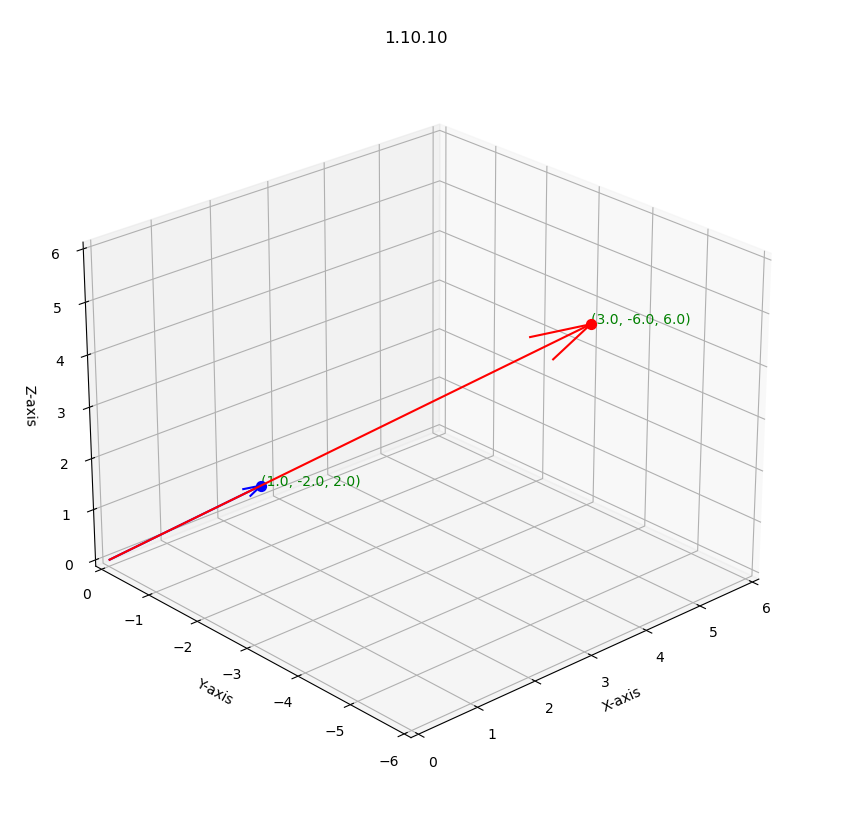
\includegraphics[width=0.6\columnwidth]{figs/fig1.png}
    \caption{Vector along given vector with specified magnitude}
    \label{3D Plot}
\end{figure}
\end{frame}
\end{document}
